\chapter{光电容积脉搏波概述}
\section{引言}
子痫前期引起孕妇机体产生的一系列病生理变化会导致机体多脏器与系统损害,最终引发全身小动脉痉挛。前人的相关研究已经证实,通过脉搏波分析技术可以实现对PE的早期筛选与检测。
前一章节受限篇幅内容仅对相关研究的结果及结论进行了介绍,并未对脉搏波进行过多的概述。故本章节将对脉搏波的产生机理、心血管血流模型及微循环血流模型等方面进行系统性介绍。
由于光电容积描述标记法在脉搏波检测采集方面具有突出优势,本论文后续研究数据均基于此法所得。因此,本章节也对光电容积描述标记法的采集原理及获得脉搏波的一般波形进行了介绍。
\section{脉搏波产生原理}
与心电产生原理类似,脉搏波也是由心脏周期性收缩与舒张引发的节律间歇性射血所产生的\cite{Allen2007},如\autoref{fig:ecgppg}所示。由于血管系统本身的阻力与弹性,射血引起的主动脉扩张与收缩最终导致血液
以压力波动的形式从主动脉传播、延伸至整个血管动脉系统。脉搏波在颈动脉、肱动脉、桡动脉等浅表动脉可以直接通过手指在皮肤表面感受到\cite{PPGYY}。
\begin{figure}[htbp]
    \centering
    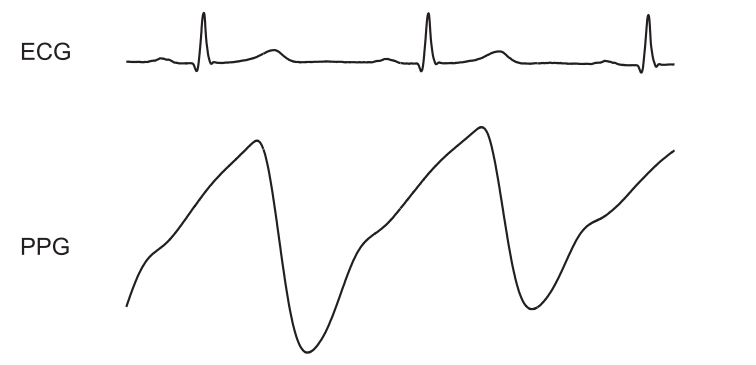
\includegraphics[width=.6\linewidth]{ch2/ecgppg}
    \caption{\label{fig:ecgppg}心电与脉搏波信号对比}
\end{figure}

脉搏波在血管动脉系统中传播时,脉搏压力波的部分能量会从不同位置反射回心脏。由于不同动脉段管壁弹性存在差异、动脉在某些部位出现分叉管以及血管本身狭窄等因素,动脉管系中会出现一系列特殊的间断点。
间断点两侧出现的阻抗突变会导致脉搏波在间断点上发生不同程度的折射和反射。动脉中向心的反射波在到达动脉瓣处后,会发生二次反射,会导致脉搏波中重搏波的出现。
这时,整个动脉管系的脉搏波传播过程可以视为这些间断点处各个行波线性叠加的结果。不同间断点处的反射特征不尽相同,其中小动脉、微动脉与毛细血管由于具有更大的阻抗,是脉搏波反射的最主要部位。

综上可知,脉搏波蕴含着丰富的血液动力学信息,可以通过脉搏波的形态、强度、速率、节律等特征反映心脏的功能与状态,也可以反映出各级动脉及分支中血管壁弹性、血管阻力、血液黏度等信息。
临床上一般将动脉系统的末梢的微动脉和微静脉之间的血液循环被称为微循环。
另一方面,根据检测方式的不同,可将脉搏波分为压力脉搏波和容积脉搏波两种类型。压力脉搏波主要表征血管内血液压力的传输,容积脉搏波主要表征外周血管与微循环中等微血管血液容积的脉动性变化。
由于光电容积脉搏波(Photoplethysmography,PPG)在观察和评估微循环状况上具有天然优势,已在动脉硬化、高血压、心肌梗塞等心脑血管疾病上有了一定的应用\cite{PPGYY,Allen2007,THOCBPM}。
\section{生理参数与非生理参数建立的微循环模型}
按照信号与系统的观点,若干相互作用、相互联系的事物按一定规律组成具有特定功能的整体均可称为系统,而信号则是反映信息的各种物理量,是系统直接进行加工、变换以实现通信的对象。而在脉搏波的工程研究领域,
人体的动脉管系亦可视为一个力学系统,心脏搏动作为该系统输入,而人体各处采集获得的脉搏波即为该系统输出(响应)。可由该系统的输入输出关系分析推断其结构特性参数,进一步研究脉搏波其他特性。\cite{PPGYY}

为尽可能精确描述心血管系统、探求心血管系统的生理特性,多年来学者们提出并建立了各种不同的数学模型进行拟合。而这些心血管模型大体上可依据建立时是否使用多个变量去拟合还原血液在血管中的可能涉及的血压、
血流弹性、阻力等生理变量分为生理参数模型与非生理参数模型两大类。生理参数模型关注心血管系统中的所有细节,模型中的各个参数变量均有较好的解释,也能与实际生理病理现象有较好的对应;而非生理参数则是
使用黑箱方法,不追求任何细节,仅通过输入输出信息来研究推导心血管系统模型,具有建立模型过程简单同时不破坏系统任何原有结构等优势。本节后续将分别从两大类模型中各选取一种经典模型进行介绍。
\subsection{双弹性腔模型及其拓展}
双弹性腔模型是心血管系统最经典的参数模型,最早由Roger M. Goldwyn等人\cite{Goldwyn1967}于1967年提出。
双弹性腔模型将人体主动脉及其分支看成两个串联的弹性腔,以表征血管系统的不同压力,同时在两个腔体之间加入了表示血液惯性的部件,如\autoref{fig:double}所示。
其中,第一个弹性腔$C_{1}$表征着主动脉及其主要分支的集总顺应性;第二个弹性腔$C_{2}$表征腹主动脉及其主要分支的集总顺应性;连接两腔体的部件$L$表征着血液惯性。
血液$q_{in}$先后流经弹性腔$C_{1}$与部件$L$,而后经过弹性腔$C_{2}$,最后流经外周阻力$R$进入静脉腔。
\begin{figure}[htbp]
    \centering
    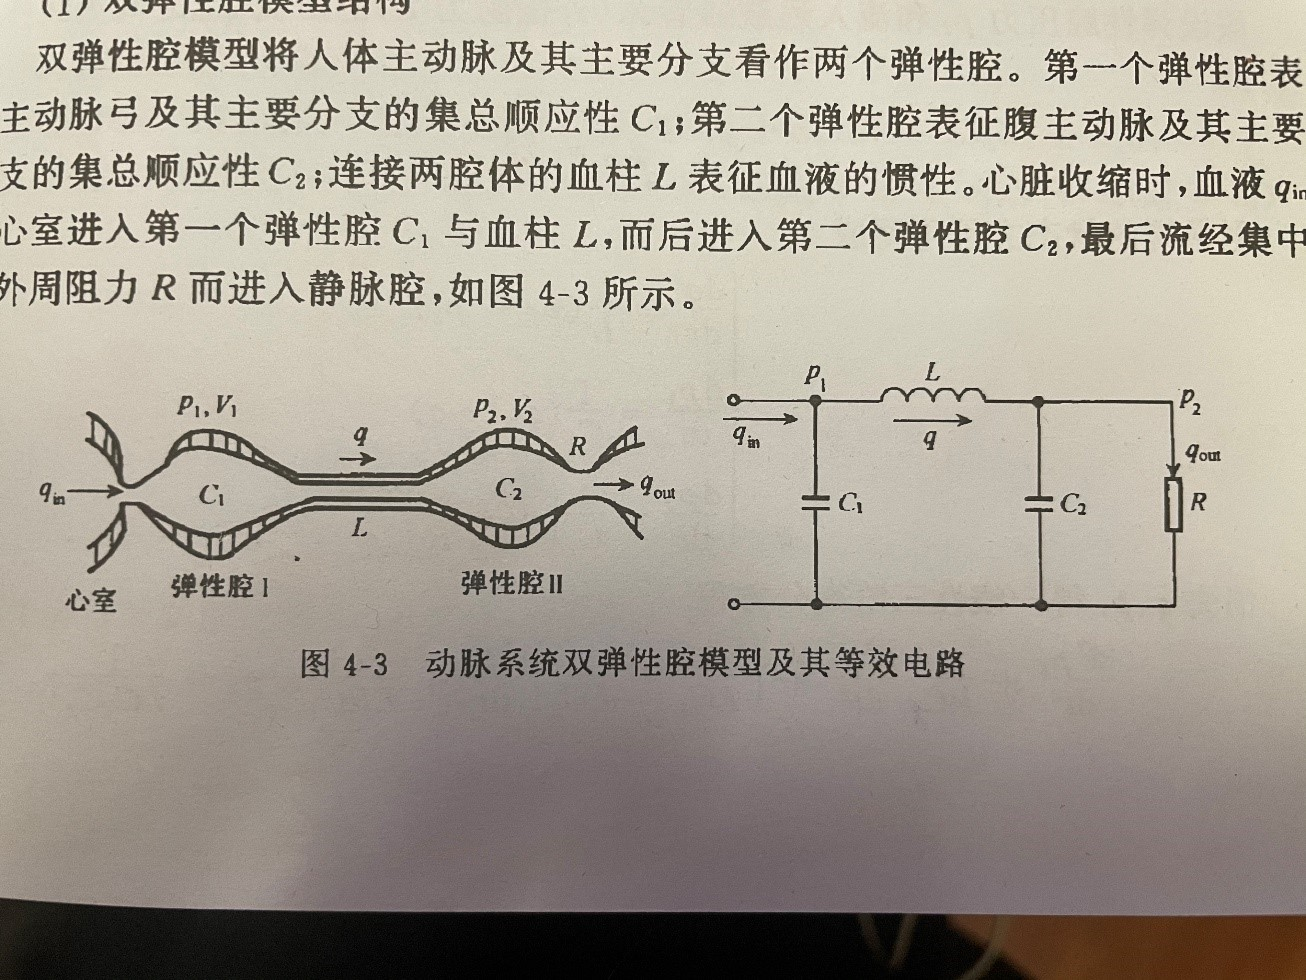
\includegraphics[width=.6\linewidth]{ch2/double}
    \caption{\label{fig:double}动脉系统双弹性腔模型及其等效电路}
\end{figure}

对于第一个弹性腔室,血液输入输出关系满足:
\begin{equation}
    \label{equ:QS1}
    q_{in}-q=\frac{\mathrm{d} V_{1}}{\mathrm{d} t}
\end{equation}
对于第一个弹性腔室,血液输入输出关系满足:
\begin{equation}
    \label{equ:QS2}
    q-q_{out}=\frac{\mathrm{d} V_{2}}{\mathrm{d} t}
\end{equation}
设腔室容积$V$与压力$p$之间为线性关系,则有:
\begin{equation}
    \label{equ:QSV1}
    \frac{\mathrm{d} V_{1}}{\mathrm{d} t}
    =\frac{\mathrm{d} V_{1}}{\mathrm{d} p_{1}}\frac{\mathrm{d} p_{1}}{\mathrm{d} t}
    =c_{1}\frac{\mathrm{d} p_{1}}{\mathrm{d} t}
\end{equation}
\begin{equation}
    \label{equ:QSV2}
    \frac{\mathrm{d} V_{2}}{\mathrm{d} t}
    =\frac{\mathrm{d} V_{2}}{\mathrm{d} p_{2}}\frac{\mathrm{d} p_{2}}{\mathrm{d} t}
    =c_{2}\frac{\mathrm{d} p_{2}}{\mathrm{d} t}
\end{equation}
不失一般性,设腔体1、2之间的血液流淌在长度为$l$,截面积为$A$的刚性管道之中。依据动量守恒,则有:
\begin{equation}
    \label{equ:QM}
    \frac{\mathrm{d}}{\mathrm{d} t}\left ( \rho Al\frac{q}{A} \right )=p_{1}A-p_{2}A
\end{equation}
其中,$\rho$为血液密度,$q$为容积流量,$q/A$为血流速度。
\autoref{equ:QM}可进一步简化为
\begin{equation}
    \left \{
    \begin{aligned}
        L\frac{\mathrm{d} q}{\mathrm{d} t} &= p_{1}-p_{2} \\
        L &=\rho \frac{l}{A} \text{(血流惯性)}
    \end{aligned}
    \right.
\end{equation}
设弹性腔压力$p_{2}$和流入血管床的血流$q_{out}$之间为线性关系,即
\begin{equation}
    \label{equ:pq}
    q_{out}=\frac{p_{2}}{R}
\end{equation}
则系统的状态方程可写成
\begin{equation}
    \left \{
    \begin{aligned}
        \frac{\mathrm{d} q}{\mathrm{d} t} &= \frac{1}{L}(p_{1}-p_{2}) \\
        \frac{\mathrm{d} p_{1}}{\mathrm{d} t} &= \frac{1}{C_{1}}(q_{in}-q) \\
        \frac{\mathrm{d} p_{2}}{\mathrm{d} t} &= \frac{1}{C_{2}}(q-\frac{p_{2}}{R}) \\
    \end{aligned}
    \right.
\end{equation}
进一步化简,消除$q$、$p_{1}$可得到:
\begin{equation}
    \label{equ:diff}
    \frac{\mathrm{d^3} p_{2}}{\mathrm{d} t^3}+\frac{1}{RC_{2}}\frac{\mathrm{d}^2p_{2} }{\mathrm{d} t^2}+
    (\frac{1}{LC_{1}}+\frac{1}{LC_{2}})\frac{\mathrm{d} p_{2}}{\mathrm{d} t}+\frac{1}{LRC_{1}C_{2}}p_{2}
    =\frac{1}{LC_{1}C_{2}}q_{in}
\end{equation}
求解该线性三阶微分方程的特征方程,可得
\begin{equation}
    \label{equ:character}
    S^3+\frac{1}{RC_{2}}S^2+(\frac{1}{LC_{1}}+\frac{1}{LC_{2}})S+\frac{1}{LRC_{1}C_{2}}=0
\end{equation}
\textbf{该特征方程的解由三个分量组成,即直流分量、非震荡衰减分量和震荡衰减分量三部分,可对脉搏波的主波、潮波和重博波等主要特征点进行较好的描绘。}

微循环容积脉搏血流模型是刘静纨等人\cite{Liu2001}在双弹性腔模型上修正、补充而来。微循环容积脉搏血流模型着重关注了弹性腔中较为笼统的外周阻力,对其进行了进一步的建模,增加了一个
由参数$R$、$L$、$C$组成的二阶系统,如\autoref{fig:micro}所示。
\begin{figure}[htbp]
    \centering
    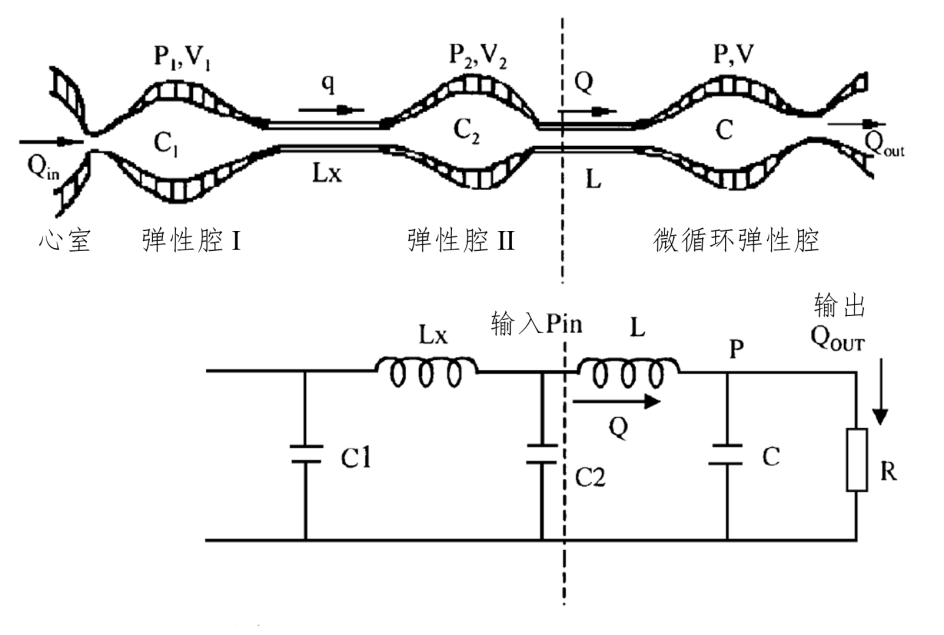
\includegraphics[width=.6\linewidth]{ch2/micro}
    \caption{\label{fig:micro}微循环容积脉搏血流模型}
\end{figure}

根据输入输出关系及该过程中动量守恒,可到微循环弹性腔血流模型的数学表达式为
\begin{equation}
    \label{equ:wxh1}
    \left \{
    \begin{aligned}
        \frac{\mathrm{d} Q}{\mathrm{d} t} &=\frac{P_{in}-P}{L}\\
        \frac{\mathrm{d} P}{\mathrm{d} t} &=\frac{Q-Q_{out}}{C}\\
        Q_{out} &=\frac{P}{R}
    \end{aligned}
    \right.
\end{equation}
消去$P$、$Q$,同样可得一线性三阶微分方程:
\begin{equation}
    \label{equ:wxh2}
    \frac{\mathrm{d^2} Q_{out}}{\mathrm{d} t^2}+\frac{1}{RC}\frac{\mathrm{d} Q_{out}}{\mathrm{d} t}+\frac{1}{LC}Q_{out}=\frac{1}{RLC}P_{in}
\end{equation}
与\autoref{equ:character}类似,这里也可以得到该微分方程的特征方程:
\begin{equation}
    \label{equ:character2}
    S^2+\frac{1}{LC}S+\frac{1}{LC}=0
\end{equation}
易得其传递函数为
\begin{equation}
    \label{equ:hs}
    \begin{aligned}
    G(s) &=\frac{Q_{out}(s)}{P_{in}(s)}=\frac{\frac{1}{RLC}}{S^2+\frac{1}{RC}S+\frac{1}{LC}} \\
    &=\frac{1}{RLC}\frac{1}{2\sqrt{(\frac{1}{2RC})^2-\frac{1}{LC}}}(\frac{1}{S-S_{1}}-\frac{1}{S-S_{2}})
    \end{aligned}
\end{equation}
其中,
\begin{equation}
    \label{equ:ss}
    \left \{
    \begin{aligned}
        S_{1} &= -\frac{1}{2RC}+\sqrt{(\frac{1}{2RC})^2-\frac{1}{LC}}\\
        S_{2} &= -\frac{1}{2RC}-\sqrt{(\frac{1}{2RC})^2-\frac{1}{LC}}\\
    \end{aligned}
    \right.
\end{equation}

\subsection{自回归滑动平均模型}
由于脉搏波信号具有较强的随机性,且其时变特性符合平稳随机信号的定义,因此,我们可以采用平稳随机信号的线性模型对脉搏波进行建模分析\cite{TJXHCL,PPGYY,Ma2015}。在此基础上,脉搏波信号$X(n)$可以看作是某一线性系统在
白噪声$W(n)$的激励下而得到的响应。只要确定了白噪声的相关参数,我们便可以将对平稳随机信号PPG的研究转换成对随机信号的线性系统的研究,典型的随机信号参数模型如\autoref{fig:eq}所示。
\begin{figure}[htbp]
    \centering
    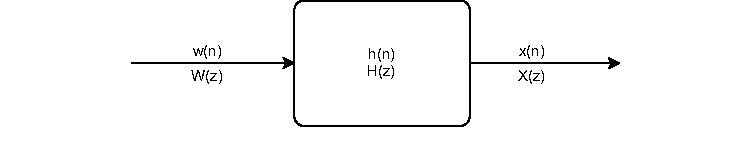
\includegraphics[width=.8\linewidth]{ch2/eq}
    \caption{\label{fig:eq}随机信号的参数模型}
\end{figure}

根据系统传递函数形式的不同,可以将平稳随机信号的线性参数模型分为滑动平均(moving average,MA)模型,自回归(autoregressive,AR)模型及自回归滑动平均模型(autoregressive moving average,ARMA)模型等三种。其中,
ARMA模型是AR模型与MA模型的组合,表示脉搏波信号$X(n)$是由自身若干过去值$X(n-k)$与激励时的白噪声$W(n)$及若干白噪声过去值$W(n-k)$线性组合产生的,即:
\begin{equation}
    \label{equ:ARMA}
    X(n)=-\sum_{k=1}^{p}a_{k}X(n-k)+\sum_{k=0}^{q}b_{k}W(n-k)
\end{equation}
对\autoref{equ:ARMA}进行$z$变换,则可得到ARMA模型的传递函数为:
\begin{equation}
    \label{equ:ARMAH}
    H(Z)=\frac{X(Z)}{W(Z)}=\frac{\sum_{k=0}^{q}b_{k}Z^{-k}}{1+\sum_{k=1}^{p}a_{k}Z^{-k}}=\frac{B(Z)}{A(Z)}
\end{equation}
可知,ARMA模型既有零点,也有极点,是零极点模型,一般记作$ARMA_{(p,q)}$,其中$p$与$q$分别是AR模型与MA模型的阶次。
对\autoref{equ:ARMA}进行傅里叶变换,可进一步得到ARMA模型的功率谱估计为\cite{TJXHCL}:
\begin{equation}
    \label{equ:ARMAP}
    \hat{P}_{ARMA}(e^{j\omega} )=
    \delta _{\omega}^2\left |  \frac{\sum_{k=0}^{p}\hat{b}_{k}e^{-j\omega}}{\sum_{k=0}^{q}\hat{a}_{k}e^{-j\omega}}\right |^2
    =\delta _{\omega}^2\left |  \frac{\hat{B(e^{j\omega} )}}{\hat{A}(e^{j\omega} )}\right |^2
\end{equation}

与上小节中的双弹性腔三阶模型类似,实际证明当采用ARMA的三阶模型$ARMA_{(3,2)}$来拟合实际脉搏波波形时,模型输出与实测波形拟合度高、误差小\cite{PPGYY}。在此情形下,脉搏波波形可由源自\autoref{equ:ARMA}的
\begin{equation}
    \label{equ:ARMA32}
    \begin{aligned}
        X(n)=&-a_{1}X(n-1)-a_{2}X(n-2)-a_{3}X(n-3)\\
        &+b_{0}W(n)+b_{1}X(n-1)+b_{2}W(n-2)
    \end{aligned}
\end{equation}
来表征。则模型的传递函数为
\begin{equation}
    \label{equ:ARMAH32}
    \begin{aligned}
        H(Z)&=\frac{X(Z)}{W(Z)}=\frac{b_{0}+b_{1}Z^{-1}+b_{2}Z^{-2}}{1+a_{1}Z^{-1}+a_{2}Z^{-2}+a_{3}Z^{-3}}\\
        &=g_{0}+g_{1}Z^{-1}+g_{2}Z^{-2}+...+g_{N-1}Z^{N-1}
    \end{aligned}
\end{equation}
其中,$g_{i}$为脉搏波实际采样数值,$N$为采样点数。
此时,求解模型则转换成求解\autoref{equ:ARMA32}中相应的$a_{i}$、$b_{i}$,使模型拟合曲线与原曲线均方差和最小,即满足:
\begin{equation}
    \label{equ:MeanSum}
    \Delta_{min}=\sum_{i=1}^{N}\left |  (g_i-g'_i)^2\right |
\end{equation}
其中$g'_i$为模型拟合数值。

\section{光电容积脉搏波采集原理}
PPG最早于1938年由Hertzman等人提出,是利用光电转换方法检测组织中血液容积变化的一种技术。由于采集测量过程无创、无痛、迅速、便捷等特性,PPG技术已经在临床
普及,成为各种监护设备必备的监测参数之一\cite{ldl,lhc}。

PPG检测可依据光的接收方式分为透射式与反射式两种\cite{THOCBPM},透射式PPG采集原理是使用一定波长光源照射在人体组织表面,由于皮肤、血液、肌肉等各组织的吸收,一部分光发生漫反射,
一部分投过组织被传感器接收,其中光源与传感器对称分布;反射式工作原理与透射式基本相同,区别在于传感器被放置光源同侧接收漫反射回来的光\cite{THOCBPM,mmt},如\autoref{fig:led}所示。
透射式PPG检测一般多用于人体耳垂、指端等部位,反射式PPG一般多用于手腕、
胸部等其他表层血管发达区域\cite{THOCBPM}。一般认为,透射式检测更方便指示心率的时间关系,而反射式则对于血管容积变化的检测更有优势\cite{mmt}。
\begin{figure}[htb]
    \centering
    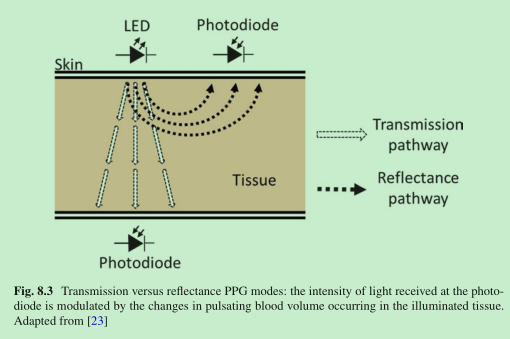
\includegraphics[width=.7\linewidth]{ch2/led}
    \caption{\label{fig:led}PPG检测的两种方式}
\end{figure}

当心脏收缩时外周血容量最多,光吸收量也最大,故检测到的光强度最小;而在心脏舒张时则恰恰相反,外周血容最小,光的吸收量最小,检测到的光强度最大\cite{lhc,cwl}。
人体耳垂、手指及脚趾等毛细血管组织发达处均可稳定采集PPG信号,同一位置左右边采集的波形高度相似,不同位置的波形略有差异\cite{Allen2000,Allen2007},如\autoref{fig:contrast}所示。
综合考虑信号质量及测量实际,指端成为了临床PPG检测位置的首选\cite{cwl}。\autoref{fig:ppgab}展示了人体指端各组织对检测光的吸收情况。
\begin{figure}[htbp]
    \centering
    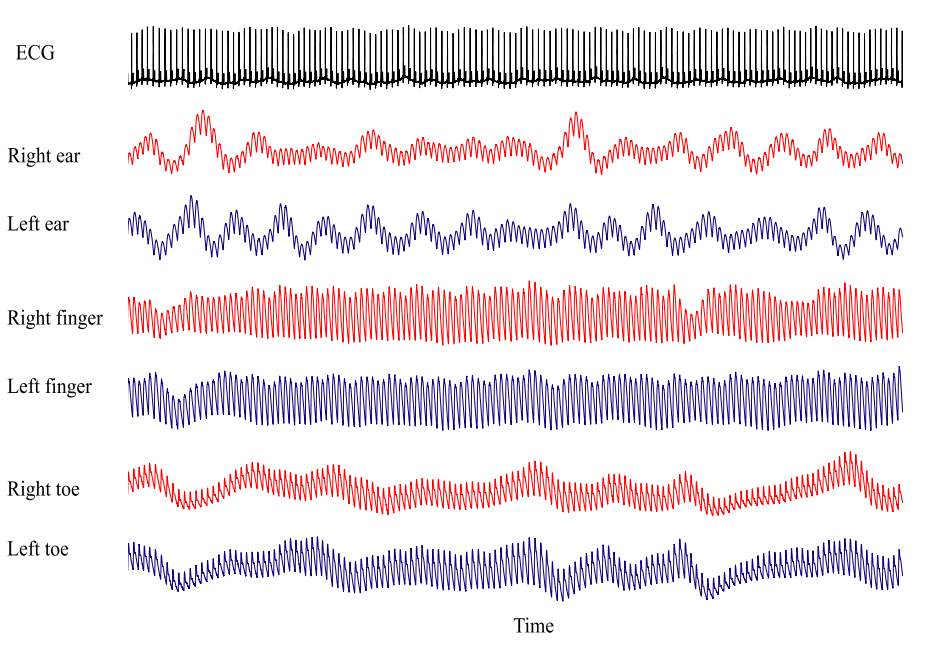
\includegraphics[width=.6\linewidth]{ch2/contrast}
    \caption{\label{fig:contrast}人体双侧多部位PPG信号对比}
\end{figure}
\begin{figure}[htb]
    \centering
    \includegraphics[width=.7\linewidth]{ch2/ppgab}
    \caption{\label{fig:ppgab}PPG信号的光吸收示意图}
\end{figure}

具体而言,物理光学中,将光通过某种透明介质后被吸收的比例定义为光的吸收度$A$,即:
\begin{equation}
    \label{equ:LBL}
    A=\lg\frac{I_{0}}{I_{T}}
\end{equation}

其中,$I_{0}$与$I_{T}$分别是入射光强度与透射光强度。而朗伯-比尔定律(Lambert-Beer's law)指出,光的吸收度与入射光的强度无关,在光程上每等厚层介质吸收相同比例值的光,即:
\begin{equation}
    \label{equ:LBL2}
    A=C \cdot \varepsilon \cdot V
\end{equation}

其中,$V$是透明介质的体积,$C$是透明介质的浓度,$\varepsilon$则是吸收系数,一般与透明介质的性质、入射光波长及温度等因素相关。

在透射式的光电检测中考虑到人体指端各组织对入射光的均有吸收,若忽略由于散射、反射等因素造成的衰减,以波长为$\lambda$的单色光垂直照射指端,则最终指端透射光强度为\cite{4122392}:
\begin{equation}
    \label{equ:AF1}
    I=I_{0}e^{-C_{t}\varepsilon _{t}V_{t}}e^{-C_{v}\varepsilon _{v}V_{v}} e^{-C_{a}\varepsilon _{a}V_{a}} 
\end{equation}

其中,下标$t$、$v$、$a$分别代表皮肤肌肉组织、静脉血液、动脉血液等成分。学者们已经证实皮肤肌肉组织、静脉血液等组织对光的吸收是恒定不变的\cite{1980Spectrophotometric,4122392}。
因此,可对\autoref{equ:AF1}进行精简,以表示通过动脉血液的透光强度\cite{PPGYY}:
\begin{equation}
    \label{equ:AF2}
    I=I_{0}e^{-C_{a}\varepsilon _{a}V_{a}} 
\end{equation}

当动脉血液的容积因心脏搏动而发生极小的变化$\Delta V_{a}$时,透光强度也将随之变动,将其记为$\Delta I$,则\autoref{equ:AF2}可改写为:
\begin{equation}
    \label{equ:AF3}
    I+\Delta I=I_{0}e^{-C_{a}\varepsilon _{a}(V_{a}+\Delta V_{a})} 
\end{equation}

将\autoref{equ:AF2}与\autoref{equ:AF3}相除,可得:
\begin{equation}
    \label{equ:AF4}
    \frac{I+\Delta I}{I}=\frac{I_{0}e^{-C_{a}\varepsilon _{a}(V_{a}+\Delta V_{a})}}{I_{0}e^{-C_{a}\varepsilon _{a}V_{a}}}=e^{-C_{a}\varepsilon _{a}\Delta V_{a}} 
\end{equation}

进一步,对\autoref{equ:AF4}两边同时取对数,并根据数学近似关系,若$x\rightarrow 0$,则$\ln(1+x)\approx x$,可得:
\begin{equation}
    \label{equ:AF5}
    \frac{\Delta I}{I}=-C_{a}\varepsilon _{a}\Delta V_{a}
\end{equation}

将\autoref{equ:AF2}代入\autoref{equ:AF5},稍作整理可得:
\begin{equation}
    \label{equ:AF6}
    \frac{\Delta V_{a}}{V_{a}}=\frac{1}{\ln(I/I_{0})}\frac{\Delta I}{I}
\end{equation}

即与个体相关性强的动脉血总的光吸收系数$\varepsilon _{a}$、动脉血浓度$C_{a}$等变量最终均与指端血液容积变化率无关,而后者与该容积透射的光强变化率$\Delta I/I$成正比例关系,从而排除了个体差异等因素的影响
\cite{1980Spectrophotometric,4122392,PPGYY}。PPG信号检测正是依此原理,通过光电转换硬件电路检测光信号并从光强变化率中获取指端血液容积变化率的信息。
\section{光电容积脉搏波的一般特征}
\subsection{时频特征}
在自回归滑动平均模型小节已经提及,PPG信号是平稳随机信号的一种。
\subsection{波形特征}
一个完整的脉搏波波形包括上升支和下降支两部分。在心脏的快速射血期,心脏收缩,血液开始进入主动脉,血管壁扩张,动脉血压快速上升,形成脉搏波的上升支。
这个过程非常迅速,因此上升支大多较为陡峭。快速射血期结束时,动脉压力达到最大,脉搏波也达到波峰,上升支结束。此后进入心室射血后期,射血速度减慢,
进入主动脉的血液容量小于从主动脉流入外周血管的血液容量,动脉开始回缩,主动脉压力减小,形成降支前段。随后心脏射血期结束,心室开始舒张,动脉血压继续下降,
直到开始下一个心动周期。下降支中可能还会出现潮波和重搏波,其波形特征与血管张力、管道阻力和血管弹性有关。脉搏波的波形特征如\autoref{fig:ppg}所示,其中A为主波波峰,
B为潮波(重搏前波),C为重搏波波谷,D为重搏波波峰,E为主波波谷。
\begin{figure}[htbp]
\centering
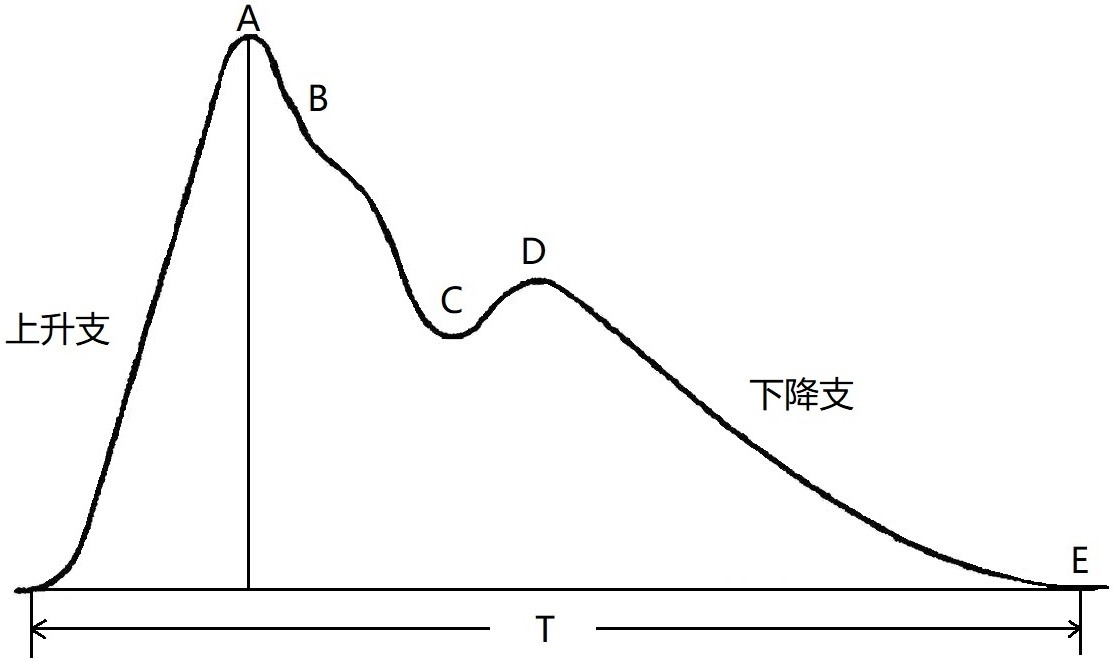
\includegraphics[width=.6\linewidth]{ch2/ppg} 
\caption{\label{fig:ppg}脉搏波波形图}
\end{figure}

\section{小结}
本章对前文中出现的脉搏波信号进行了详细的介绍,通过脉搏波产生的基本原理说明其在微循环监测领域的重要意义。其次,通过参数与非参数两种方式对脉搏波微循环系统进行了建模分析,并进一步补充了光电容积脉搏波的
检测原理。最后对光电容积脉搏波的一般性特征与波形特征进行了说明,阐述了脉搏波的基本特点。